% reset memory of all acronyms, so \ac will print out full name of acronym!
\acresetall 
\hyphenation{An-wendungs-land-schaft} % because ngerman/babel doesn´t know it correctly... 

\chapter{Einleitung}
\paragraph{Motivation der Arbeit}
Die \ac{SV} ist bestrebt ihre Versicherungsprozesse und den Kontakt mit den Kunden durch digitale Kanäle ständig zu verbessern. Die Digitalisierung ist ein wichtiger Bestandteil der \ac{SV}-Strategie: So ist sie Mitbegründerin der \enquote{id-fabrik}\footnote{Ein Start-up, das federführend Innovationen im Bereich der S-Finanzgruppe erzeugt.} und Mitglied im \enquote{InsurLab Germany}\autocite[vgl.][S.\,30]{sv_sparkassenversicherung_sv_2019}. Um den Kunden der \ac{SV} immer besseren Service bieten zu können, möchte sie die neuen Technologien nutzen. Die Nachfrage nach ständiger Verfügbarkeit der Systemen stellt die IT-Dienstleisterin (\ac{SVI}) der \ac{SV} vor neue Herausforderungen, denn die Verteilungsprozesse von neuen Versionen der Anwendungen können derzeit nicht während des laufenden Betriebes durchgeführt werden. So müssen neue Funktionen warten, bis das Wochenende des \enquote{Release} sie veröffentlicht, d.\,h. im schlechtesten Fall ist die neue Funktion drei Monate auf der Warteliste. Dieses Vorgehen passt nicht zu den digitalen Bestrebungen der \ac{SV}. Als Lösungsansatz sind die Eigenschaften der \enquote{Cloud}-Technologie zu nennen. Jedoch muss aus IT-Sicht hier eine Anmerkung gemacht werden:

\begin{figure}[h!]
	\centering
	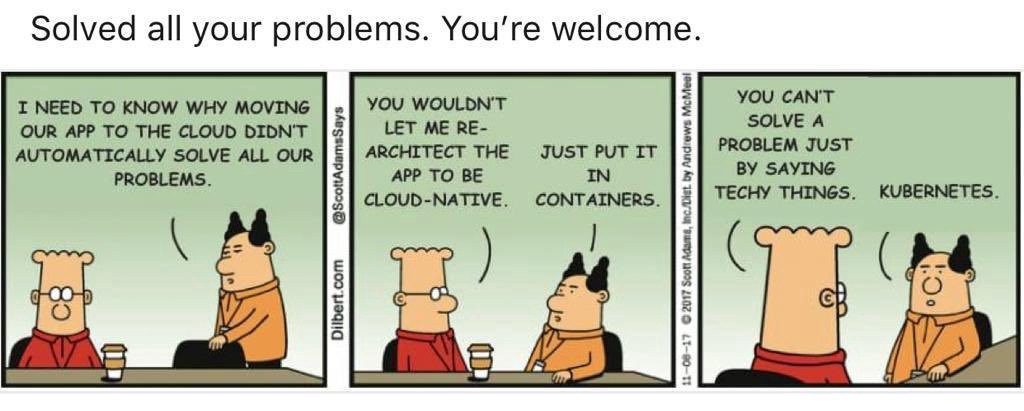
\includegraphics[scale=0.33]{img/dilbertCloud.jpeg}
	\caption{Dilbert Comic zu \textsc{Kubernetes}}
	\label{abb:dilbertK8s}
	{\footnotesize Quelle: \cite{DilbertKubernetes}\par}
	{\footnotesize Redaktionelle Anmerkung: Abbildung nur als komprimiertes Format verfügbar (Qualitätseinbuße)}
\end{figure}

Die, in Abbildung \vref{abb:dilbertK8s}, dargestellte Aussage ist absichtlich überspitzt, um das Verständnis der Lösungsmöglichkeiten der \enquote{Cloud}-Technologie zu schärfen. Der Hinweis der IT stellt klar, dass das oben beschriebene Problem nur mit einer ganzheitlichen Lösung zu erreichen ist. Es führt nicht zum gewünschten Ergebnis, Anwendungen, die nicht für die \enquote{Cloud} gedacht sind, mit Zwang in diese zu bewegen. Diese Arbeit beschreibt den Prozess zur Verteilung von Container-Anwendungen. 

\paragraph{Problemstellung/-abgrenzung}
Bei der vorliegenden Arbeit handelt es sich um eine mehrteilige Analyse und Konzeption, die bei abgeschlossener Untersuchung ein Konzept zur automatischen Verteilung von Container-Anwendungen, die Betrachtung der Effekte von diesen Anwendungen und ein Ergebnis zu den sicherheitsrelevanten Aspekten dieses Prozess enthalten wird. Dabei akkumuliert sich der Fokus die Prozessentwicklung der Verteilung einer Container-Anwendung. Des Weiteren ist die Untersuchung der Anforderungen, die Analyse der \enquote{Cloud}-Plattform \textsc{OpenShift}\footnote{\enquote{\textsc{OpenShift} is an open source container application platform by Red Hat based on the Kubernetes container orchestrator for enterprise app development and deployment.} Quelle: \cite[][]{red_hat_inc_openshift_2020}} und die Erstellung eines Generierungsalgorithmus im Fokus dieser Arbeit. Dieser Teilkomplex wird durch die Forschungsfrage eins -- Wie können Container-Anwendungen den Prozess des automatisierten \enquote{Deployments}\footnote{\enquote{Software deployment may be considered to be a process consisting of a number of inter-related activities including the release of software at the end of the development cycle; the configuration of the software, the installation of software into the execution environment, and the activation of the software. It also includes post installation activities including the monitoring, deactivation, updating, reconfiguration, adaptation, redeploying and undeploying of the software.} (\cite{dearle_software_2007})} unterstützen? -- abgedeckt. Der Anforderungskatalog soll in Zusammenarbeit mit dem Fachbereich erstellt werden, um die Akzeptanz der Anforderungen zu steigern und um die Validität dieser zu gewährleisten. Die Forschungsfragen zwei und drei (siehe dazu Paragraph \enquote{Forschungsfragen/-design}) analysieren den wirtschaftlichen und sicherheits-/rechtlich-relevanten Bereich des Themenkomplexes der Bachelorarbeit. Dabei bedient sich die Forschungsfrage zwei der Methodik des Geschäftsvorfalls (\enquote{Business Case}). Beide Forschungsfragen werden durch eine Analyse des Ist-Zustands eine initiale Konzeption ableiten. 
\par
Nicht Teil dieser Arbeit ist die unternehmensinterne Entscheidung über die Verantwortlichkeiten des zu entwickelnden Prozesses und die Erstellung einer unternehmensweiten Strategie zum Container-\enquote{Deployment}. Die Anpassung des unternehmensinternen Prozesses \enquote{Release} ist nicht Teil dieser Arbeit. Dieser übersteigt die Anforderungen, die an diese Bachelorarbeit gestellt werden. Auch genügt die rechtliche Betrachtung des Einkaufsprozess von Software nicht den juristischen Ansprüchen eines Gutachtens. Dies ist jedoch nicht Ziel der Arbeit. Die wirtschaftliche Betrachtung des Geschäftsvorfalls  \enquote{Container-Verteilung} dient als reine Veranschaulichung der Methodik und genügt nicht einer vollständigen Betrachtung, die die \ac{BWL} vorgibt. Der Fokus der Arbeit liegt auf der technischen Entwicklung eines Verteilungsprozesses.

\paragraph{Zielstellung der Arbeit}
Folgende \textit{SMART}\footnote{\enquote{SMART-Regel sind Formulierungshilfen, die eine einfache Methode zum Operationalisieren von Zielen und auch zur Überprüfung der Güte von Zielen darstellen.} Quelle: \cite[][S.69]{dechange_projektmanagement_2020}}-formulierte Ziele sollen diese Bachelorthesis leiten, messbar machen und später als Anhaltspunkt zur Evaluierung des Erfolgs dienen:

\begin{enumerate}
	\item Entwicklung eines Verteilungsprozess für einfache Container-Anwendungen bis zum 27.April 2020. Einfach bedeutet hier, dass die Container-Struktur aus einer \enquote{Base Image}\footnote{siehe dazu Kapitel \vref{kap:container}}-Schicht und einer Logik-Schnitt (Eigenentwicklung) besteht.
	\item Der Prozess muss zu 98\,\% ohne Einwirkung von Menschen während des Verteilungsvorgangs funktionieren, d.\,h. er ist (annähernd) voll automatisiert. Dies muss bis zum Ende des Bearbeitungszeitraum der Arbeit (8.Mai 2020) umgesetzt werden.
	\item Die Generierung einer Konfigurationsdatei soll in 9 von 10 Verteilungen automatisch mit einem Skript durchgeführt werden. Umzusetzen ist dies bis zum 08.Mai 2020.
	\item Die Vorteile einer Container-Anwendung für die Verteilung dieser sollen erforscht werden. Akzeptiert ist dieses Ziel, sobald eine Auflistung und eine kritische Betrachtung der Ergebnisse beschrieben wurde. Umzusetzen bis zum Ende des Bearbeitungszeitraums. (Dieses Ziel ist nicht komplett \textit{SMART}-konform, da die zumindest die Messbarkeit ohne genannte Messgröße nicht nachvollziehbar ist.)
	\item Die wirtschaftliche Betrachtung muss sich anhand des Standes von Wissenschaft und Technik orientieren. Dazu werden gängige Regeln von \cite{herman_is_2009}, \cite{brugger_it_2009} u.\,Ä. benutzt. Diese Betrachtung muss bis zum Ende des Bearbeitungszeitraums durchgeführt werden. Die Messbarkeit wird durch die Einhaltung der oben genannten Regeln beschrieben.
	\item Die sicherheits-/rechtlich-relevanten Aspekte dieses Projektes sollen anhand der, für die Finanzdienstleitungs-/Versicherungsbranche, geltenden Vorschriften beleuchtet werden. Der Umfang dieser Beleuchtung beschränkt sich auf das Nötigste, d.\,h. es müssen nur die wichtigsten Regeln beschrieben werden. Dies ist bis zum Ende des Bearbeitungszeitraumes umzusetzen. Die Messbarkeit ist durch die sicherheits-/rechtlich-relevanten Vorschriften bestimmt.
\end{enumerate}

\paragraph{Forschungsfragen/-design}\label{ffs}
Die Forschungsfragen mit der sich diese Bachelorarbeit beschäftigen wird, sind eine direkte Konsequenz aus der Zielstellung und aus den unternehmensinternen Anforderungen an einen möglichen automatisierten Prozess. Dabei liegt der Fokus auf der Betrachtung beider Teildisziplinen der Wirtschaftsinformatik, nämlich der Informatik und der Wirtschaft -- jedoch wird der größere Teil dieser Arbeit einen informationstechnischen Fokus besitzen. Die folgende Aufzählung nennt die einzelnen Forschungsfragen, die im weiteren Verlauf ein gemeinsames Ergebnis erbringen werden. Dieses ist in Kapitel \vref{kritischeBetrachtung} zu finden.
\begin{enumerate}
	\item Wie können Container-Anwendungen den Prozess des automatisierten \enquote{Deployments} unterstützen?
	\item Welche wirtschaftlichen Vorteile hat der Einsatz von Container auf den Prozess des automatisierten \enquote{Deployments}?
	\item Welche besonderen sicherheitstechnischen Aspekte muss ein solcher Prozess im Bereich der Versicherung erfüllen?
\end{enumerate}
% TODO: Nachfolgende Absätze auf Richtigkeit prüfen
Die Forschungsfrage eins wird einen Ist-Zustand analysieren. Diese Analyse enthält eine Betrachtung des Prozesses und einen Anforderungskatalog der Entwicklungsabteilungen an den zu konzeptionierenden \enquote{Deployment}-Prozess für die Container-Anwendungen. Danach wird ein Konzept eines container-basierten, automatisierten \enquote{Deployment}-Prozesses erstellt, das aus der Entwicklung dieses und einer Standardisierung der beteiligten Dateien besteht. Die Forschungsfrage eins schließt mit einem Teilergebnis ab. \par

Die Forschungsfrage zwei beschäftigt sich mit den wirtschaftlichen Vorteilen eines Einsatzes der Container auf den Prozess des automatisierten \enquote{Deployment}-Prozesses. Dabei werden die Erstellung eines \enquote{Business Case\footnote{engl. Geschäftsszenario}}, die Prüfung der Übereinstimmung der Ziele dieser Arbeit mit der Geschäftsstrategie der \ac{SVI} und mögliche Disharmonien dieser identifiziert. Außerdem entsteht eine Konzeption eines verbesserten Geschäftsszenarios, das die Kosteneinsparpotentiale und die Zielharmonisierung enthalten wird. Ein Ausblick schließt die Forschungsfrage zwei ab. 
\par
Die Forschungsfrage drei identifiziert sicherheitsrelevante Anforderungen, die nicht nur die Anwendung selbst betreffen, sondern Auswirkung auf die komplette Anwendungslandschaft (\acs{AWL}) haben. Diese Anforderungen werden durch das \acl{BSI} und verschiedene \textsc{DIN/ISO}-Normen beeinflusst. Außerdem soll analysiert werden, wie bei der Beschaffung von \enquote{open source}- bzw. \enquote{closed source}-Anwendungen mögliche Schwachstellen identifiziert werden, die potenzielle Angriffsvektoren in der \ac{AWL} eröffnen würden, und wie mit diesen verfahren wird. Dabei soll versucht werden Rückschlüsse auf die Anwendung \textsc{OpenShift} von \textsc{Red Hat\footnote{\enquote{Red Hat ist der weltweit führender Anbieter von Open Source-Lösungen, die auf verlässlichen und leistungsstarken Technologien in den Bereichen \enquote{Cloud}, Virtualisierung, Storage, Linux, Mobile und Middleware basieren. Darüber hinaus bieten wir Support-, Trainings- und Consulting-Services an, die mehrfach prämiert wurden.} Quelle: \cite[][]{red_hat_inc_red_2020}}} zu ziehen. Auch hier wird ein Teilergebnis diese Forschungsfrage abschließen


\paragraph{Einordnung der Abteilung in den Geschäftsprozess}
Die Abteilung \ac{IE2}, die sich im Bereich der Organisationseinheit \ac{IE} befindet, befasst sich in erster Linie mit dem Transport (\enquote{Deployment}) von Software-Artefakten der einzelnen Software-Produkte der \ac{SVI}. Diese werden für die \ac{SV} entwickelt, betrieben und gewartet. Zu den zentralen Aufgaben der Abteilung gehören die Planung, Durchführung und Überwachung der \enquote{Build/Deployment}-Prozesse der verschiedenen Service-Umgebungen, die aus mehreren Server-Verbünden bestehen. Des Weiteren stellt \ac{IE2} die Einspielung von datenbank-relevanten Objekten sicher. Auch entwickelt sie die Bau- und Transportprozesse kontinuierlich weiter und passt diese an die sich ständig veränderten Anforderung der Entwicklungsabteilungen an. Von zentraler Bedeutung sind die Planung und Durchführung der Veröffentlichungen der neuen Versionen einer zu betreuenden Anwendung. Zu dieser Aufgabe gehören auch Aufbau und Bereitstellung der Systemtest-, Releasetest- und Produktionsumgebungen. Eine weitere zentrale Aufgabe ist das Umgebungsmanagement. Die Aufgaben dieses Teilbereichs befassen sich mit folgenden Inhalten: Planung von Aktivitäten in der Produktionsumgebung, Planung und Koordination der Infrastruktur und Notfall-\enquote{Fix} der Produktion, der allgemeinen \enquote{Patch}-Planung; Beratung zur Erweiterung, Koordination und Planung von verschiedenen Testumgebungen. Außerdem ist das Umgebungsmanagement Teil des \ac{CAB}, das ein Gremium nach der Sammlung \ac{ITIL} darstellt. Dieses ist für die Freigabe von \enquote{Changes} verantwortlich und hat ständige, wie auch der Situation angepasste, Mitglieder. 

\paragraph{Aufbau der Arbeit}
In Kapitel \vref{ff1} wird die Forschungsfrage eins behandelt. Diese beschreibt grundlegende Aspekte der Anforderungsanalyse, des \acl{Cloud-C} und der Container(-isierung)/Orchestrierung. Diese Grundlagen werden später benutzt, um das Vorgehen in diesem Kapitel nachvollziehbar zu gestalten. Die Anforderungsanalyse erkundet die Wünsche der Fachbereiche im Bezug auf die Verteilung von Container-Anwendungen und entwickelt daraus Anforderungen, die dem Stand der Wissenschaft genügen. Wichtig in diesem Kapitel ist die Entwicklung des Prozesses und die damit verbundene Beschreibung der Tätigkeiten.
\par
In Kapitel \vref{ff2} wird die Forschungsfrage zwei behandelt:
\par
In Kapitel \vref{ff3} wird die Forschungsfrage drei behandelt: 
\par
In Kapitel \vref{kritischeBetrachtung} 
